\documentclass[tikz,border=10pt]{standalone}
\usepackage{tikz}
\usepackage{amsmath}
\usepackage{amssymb}
\usetikzlibrary{shapes.geometric, arrows, positioning, fit, backgrounds}

% 문서 참조 정보 매핑
% Section 34.1: Basic Components (식 34.1-34.6)
% Section 34.2: Image-Based Visual Servo (식 34.7-34.12)
% Section 34.2.1: Interaction Matrix (식 34.11-34.12)
% Section 34.2.2: Approximating Interaction Matrix

\begin{document}
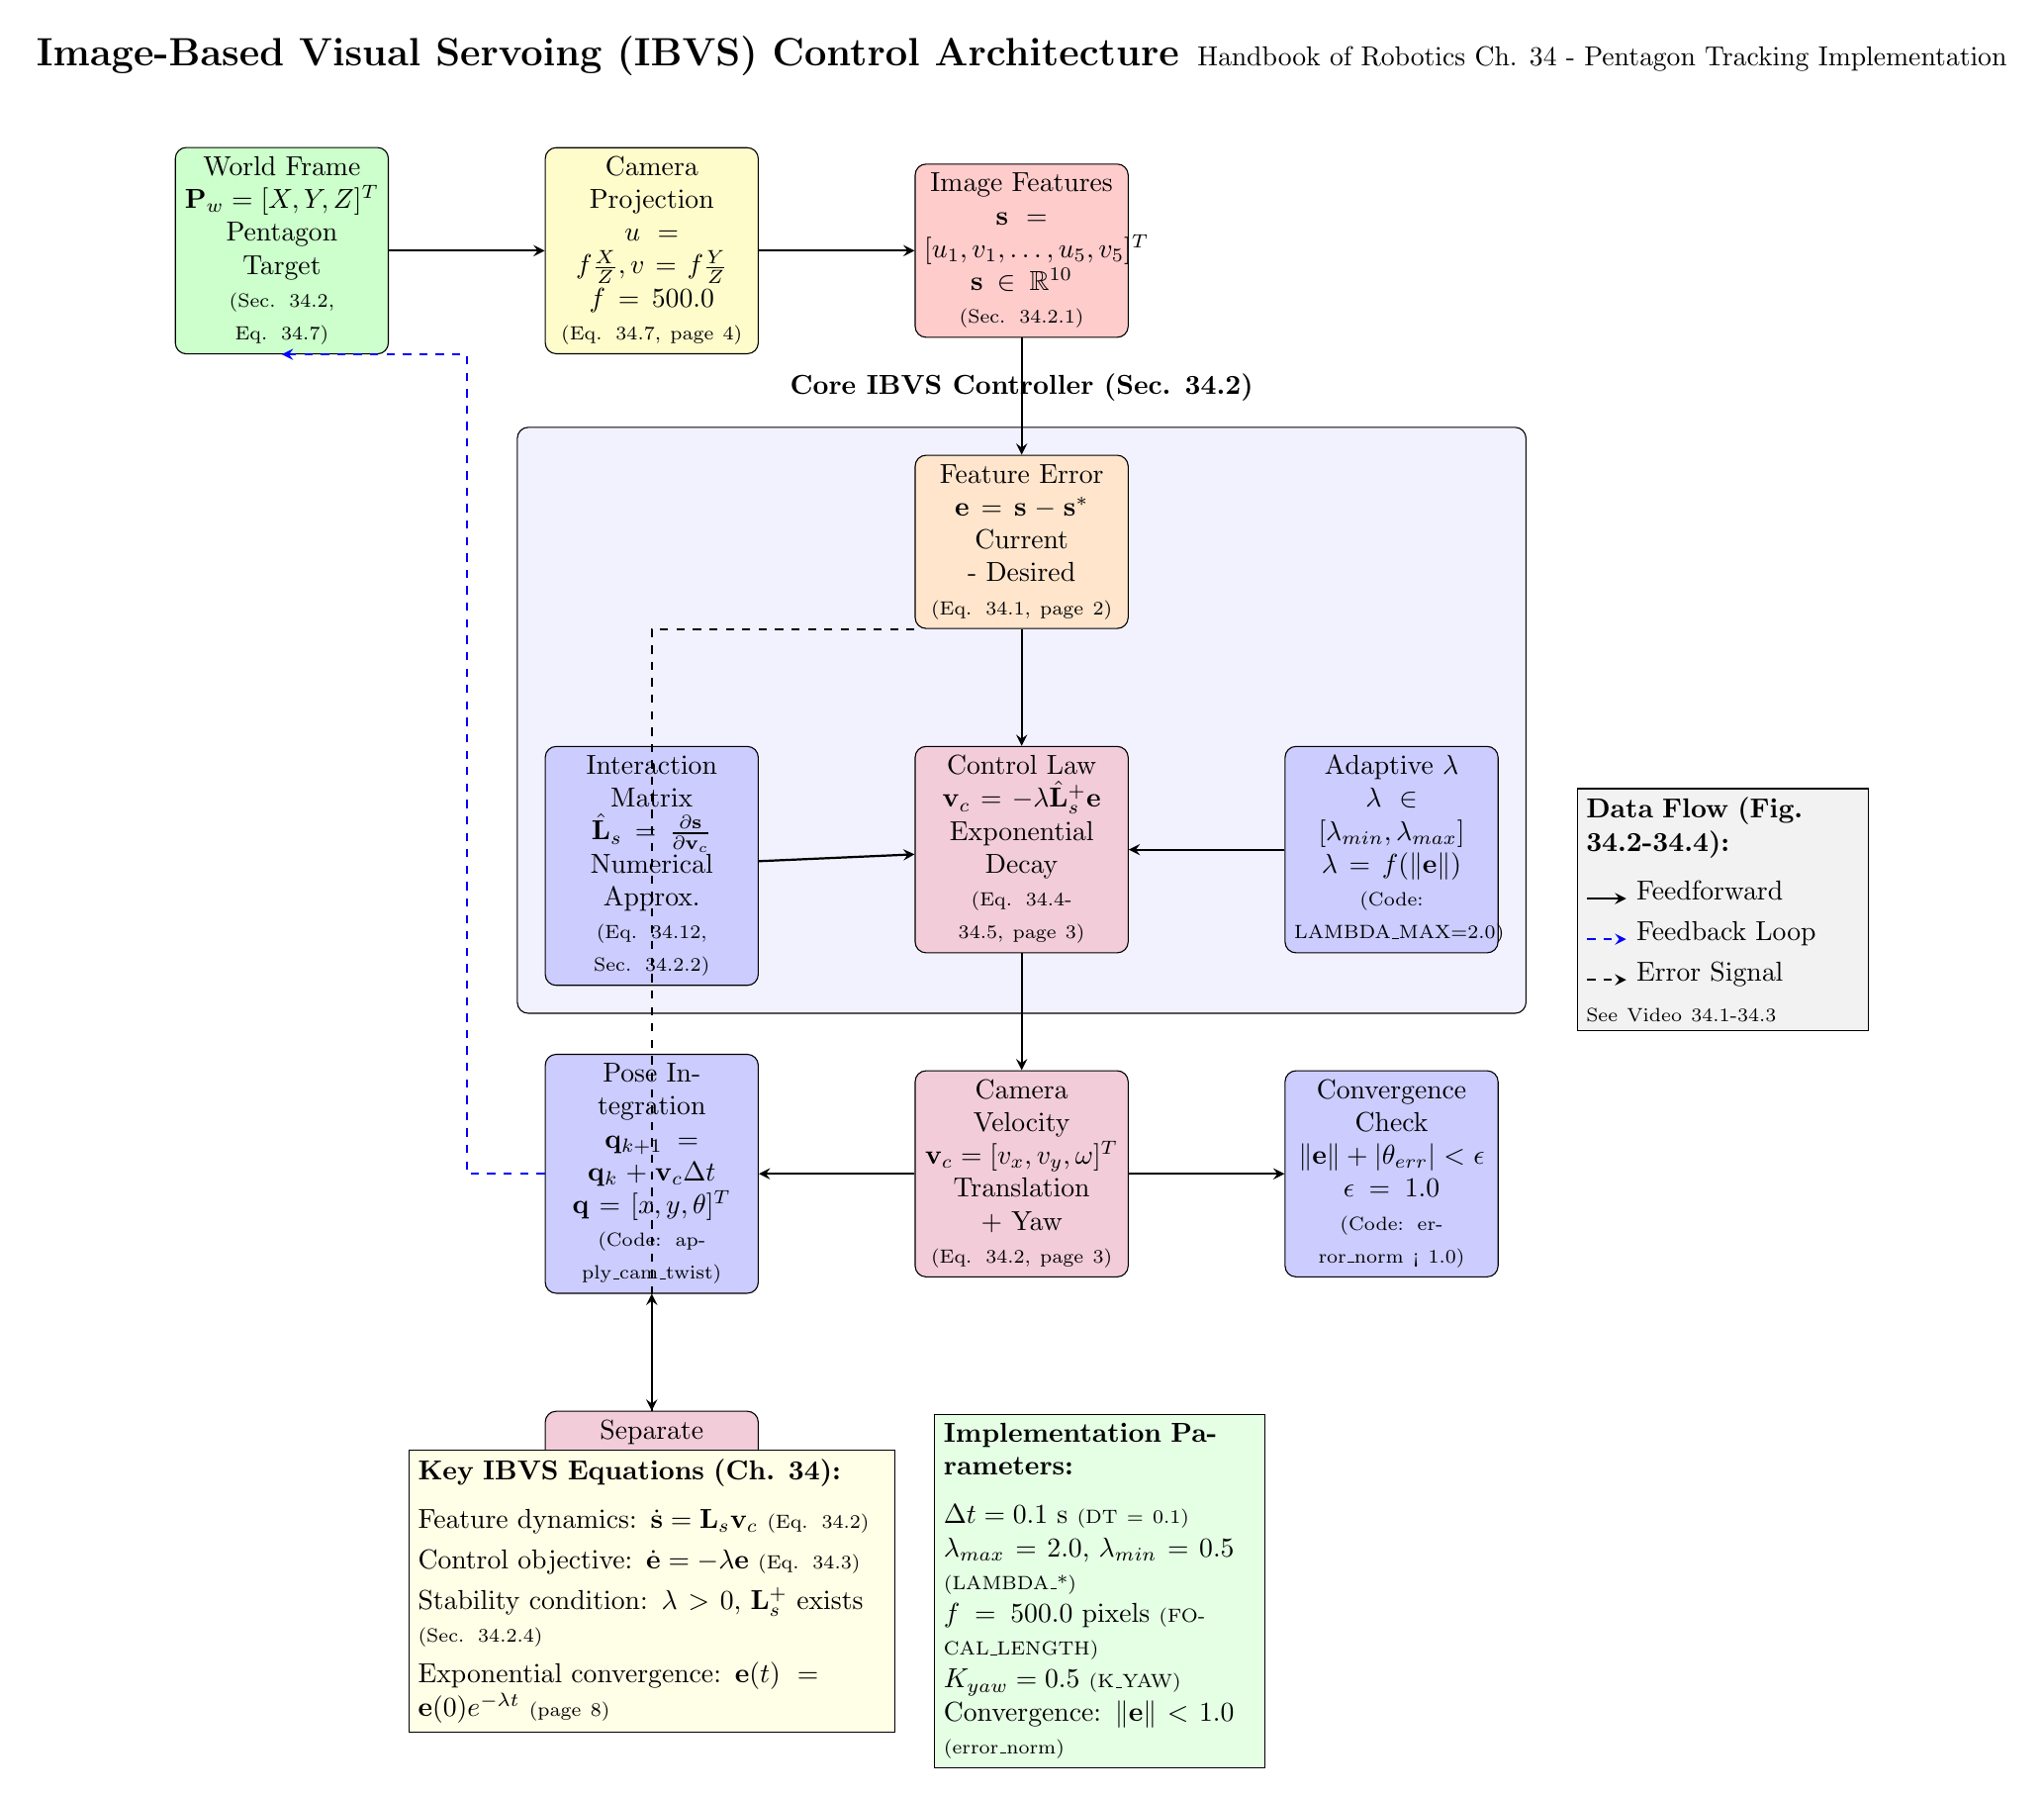
\begin{tikzpicture}[
    node distance=1.5cm and 2cm,
    block/.style={rectangle, draw, fill=blue!20, text width=2.5cm, text centered, rounded corners, minimum height=1cm},
    world/.style={rectangle, draw, fill=green!20, text width=2.5cm, text centered, rounded corners, minimum height=1cm},
    camera/.style={rectangle, draw, fill=yellow!20, text width=2.5cm, text centered, rounded corners, minimum height=1cm},
    image/.style={rectangle, draw, fill=red!20, text width=2.5cm, text centered, rounded corners, minimum height=1cm},
    control/.style={rectangle, draw, fill=purple!20, text width=2.5cm, text centered, rounded corners, minimum height=1cm},
    error/.style={rectangle, draw, fill=orange!20, text width=2.5cm, text centered, rounded corners, minimum height=1cm},
    arrow/.style={thick,->,>=stealth}
]

% Main blocks with document references
\node[world] (world) {World Frame\\$\mathbf{P}_w = [X, Y, Z]^T$\\Pentagon Target\\{\scriptsize (Sec. 34.2, Eq. 34.7)}};
\node[camera, right=of world] (projection) {Camera Projection\\$u = f\frac{X}{Z}, v = f\frac{Y}{Z}$\\$f = 500.0$\\{\scriptsize (Eq. 34.7, page 4)}};
\node[image, right=of projection] (features) {Image Features\\$\mathbf{s} = [u_1, v_1, \ldots, u_5, v_5]^T$\\$\mathbf{s} \in \mathbb{R}^{10}$\\{\scriptsize (Sec. 34.2.1)}};

\node[error, below=of features] (error_calc) {Feature Error\\$\mathbf{e} = \mathbf{s} - \mathbf{s}^*$\\Current - Desired\\{\scriptsize (Eq. 34.1, page 2)}};

\node[block, below left=of error_calc] (interaction) {Interaction Matrix\\$\hat{\mathbf{L}}_s = \frac{\partial \mathbf{s}}{\partial \mathbf{v}_c}$\\Numerical Approx.\\{\scriptsize (Eq. 34.12, Sec. 34.2.2)}};

\node[control, below=of error_calc] (control_law) {Control Law\\$\mathbf{v}_c = -\lambda \hat{\mathbf{L}}_s^+ \mathbf{e}$\\Exponential Decay\\{\scriptsize (Eq. 34.4-34.5, page 3)}};

\node[block, below right=of error_calc] (lambda_adapt) {Adaptive $\lambda$\\$\lambda \in [\lambda_{min}, \lambda_{max}]$\\$\lambda = f(\|\mathbf{e}\|)$\\{\scriptsize (Code: LAMBDA\_MAX=2.0)}};

\node[control, below=of control_law] (velocity) {Camera Velocity\\$\mathbf{v}_c = [v_x, v_y, \omega]^T$\\Translation + Yaw\\{\scriptsize (Eq. 34.2, page 3)}};

\node[block, left=of velocity] (integration) {Pose Integration\\$\mathbf{q}_{k+1} = \mathbf{q}_k + \mathbf{v}_c \Delta t$\\$\mathbf{q} = [x, y, \theta]^T$\\{\scriptsize (Code: apply\_cam\_twist)}};

\node[block, right=of velocity] (convergence) {Convergence Check\\$\|\mathbf{e}\| + |\theta_{err}| < \epsilon$\\$\epsilon = 1.0$\\{\scriptsize (Code: error\_norm < 1.0)}};

% Additional control blocks
\node[control, below=of integration] (yaw_control) {Separate Yaw Control\\$\omega = -K_{yaw} \theta_{err}$\\$K_{yaw} = 0.5$\\{\scriptsize (Code: K\_YAW = 0.5)}};

% Arrows
\draw[arrow] (world) -- (projection);
\draw[arrow] (projection) -- (features);
\draw[arrow] (features) -- (error_calc);
\draw[arrow] (error_calc) -- (control_law);
\draw[arrow] (interaction) -- (control_law);
\draw[arrow] (lambda_adapt) -- (control_law);
\draw[arrow] (control_law) -- (velocity);
\draw[arrow] (velocity) -- (integration);
\draw[arrow] (velocity) -- (convergence);

% Feedback loop
\draw[arrow, dashed, thick, blue] (integration.west) -| ++(-1,0) |- (world.south);
\draw[arrow] (yaw_control) -- (integration);

% Error feedback to yaw control
\draw[arrow, dashed] (error_calc.south west) -| (yaw_control.north);

% Add mathematical formulations in boxes with references
\node[draw, fill=yellow!10, text width=6cm, below=2cm of integration] (equations) {
\textbf{Key IBVS Equations (Ch. 34):}\\[0.2cm]
Feature dynamics: $\dot{\mathbf{s}} = \mathbf{L}_s \mathbf{v}_c$ {\scriptsize (Eq. 34.2)}\\[0.1cm]
Control objective: $\dot{\mathbf{e}} = -\lambda \mathbf{e}$ {\scriptsize (Eq. 34.3)}\\[0.1cm]
Stability condition: $\lambda > 0$, $\mathbf{L}_s^+$ exists {\scriptsize (Sec. 34.2.4)}\\[0.1cm]
Exponential convergence: $\mathbf{e}(t) = \mathbf{e}(0) e^{-\lambda t}$ {\scriptsize (page 8)}
};

% Add parameter box with code references
\node[draw, fill=green!10, text width=4cm, right=0.5cm of equations] (parameters) {
\textbf{Implementation Parameters:}\\[0.2cm]
$\Delta t = 0.1$ s {\scriptsize (DT = 0.1)}\\
$\lambda_{max} = 2.0$, $\lambda_{min} = 0.5$ {\scriptsize (LAMBDA\_*)}\\
$f = 500.0$ pixels {\scriptsize (FOCAL\_LENGTH)}\\
$K_{yaw} = 0.5$ {\scriptsize (K\_YAW)}\\
Convergence: $\|\mathbf{e}\| < 1.0$ {\scriptsize (error\_norm)}
};

% Add title with document reference
\node[above=1cm of features, font=\Large\bfseries] (title) {
Image-Based Visual Servoing (IBVS) Control Architecture\\
{\normalsize\normalfont \ \ Handbook of Robotics Ch. 34 - Pentagon Tracking Implementation}
};

% Background for main control loop with reference
\begin{scope}[on background layer]
\node[draw, fill=blue!5, fit=(error_calc)(control_law)(interaction)(lambda_adapt), 
      inner sep=10pt, rounded corners] (control_group) {};
\node[above=0.2cm of control_group.north, font=\bfseries] {Core IBVS Controller (Sec. 34.2)};
\end{scope}

% Add data flow legend with document context
\node[draw, fill=gray!10, text width=3.5cm, above right=0.5cm and 1cm of convergence] (legend) {
\textbf{Data Flow (Fig. 34.2-34.4):}\\[0.2cm]
\tikz\draw[arrow] (0,0) -- (0.5,0); Feedforward\\[0.1cm]
\tikz\draw[arrow, dashed, blue] (0,0) -- (0.5,0); Feedback Loop\\[0.1cm]
\tikz\draw[arrow, dashed] (0,0) -- (0.5,0); Error Signal\\[0.1cm]
{\scriptsize See Video 34.1-34.3}
};

\end{tikzpicture}
\end{document}
